\documentclass[11pt]{article}

\usepackage{epsfig}
\usepackage{amsfonts}
\usepackage{amssymb}
\usepackage{amstext}
\usepackage{amsmath}
\usepackage{xspace}
\usepackage{theorem}
\usepackage{times}
\usepackage{graphicx}

%\usepackage{layout}% if you want to see the layout parameters
                     % and now use \layout command in the body

% This is the stuff for normal spacing
\makeatletter
 \setlength{\textwidth}{6.5in}
 \setlength{\oddsidemargin}{0in}
 \setlength{\evensidemargin}{0in}
 \setlength{\topmargin}{0.25in}
 \setlength{\textheight}{8.25in}
 \setlength{\headheight}{0pt}
 \setlength{\headsep}{0pt}
 \setlength{\marginparwidth}{59pt}

 \setlength{\parindent}{0pt}
 \setlength{\parskip}{5pt plus 1pt}
 \setlength{\theorempreskipamount}{5pt plus 1pt}
 \setlength{\theorempostskipamount}{0pt}
 \setlength{\abovedisplayskip}{8pt plus 3pt minus 6pt}

 \renewcommand{\section}{\@startsection{section}{1}{0mm}%
                                   {2ex plus -1ex minus -.2ex}%
                                   {1.3ex plus .2ex}%
                                   {\normalfont\Large\bfseries}}%
 \renewcommand{\subsection}{\@startsection{subsection}{2}{0mm}%
                                     {1ex plus -1ex minus -.2ex}%
                                     {1ex plus .2ex}%
                                     {\normalfont\large\bfseries}}%
 \renewcommand{\subsubsection}{\@startsection{subsubsection}{3}{0mm}%
                                     {1ex plus -1ex minus -.2ex}%
                                     {1ex plus .2ex}%
                                     {\normalfont\normalsize\bfseries}}
 \renewcommand{\paragraph}{\@startsection{paragraph}{4}{0mm}%
                                    {1ex \@plus1ex \@minus.2ex}%
                                    {-1em}%
                                    {\normalfont\normalsize\bfseries}}
 \renewcommand{\subparagraph}{\@startsection{subparagraph}{5}{\parindent}%
                                       {2.0ex \@plus1ex \@minus .2ex}%
                                       {-1em}%
                                      {\normalfont\normalsize\bfseries}}
\makeatother

\newenvironment{proof}{{\bf Proof:  }}{\hfill\rule{2mm}{2mm}}
\newenvironment{proofof}[1]{{\bf Proof of #1:  }}{\hfill\rule{2mm}{2mm}}
\newenvironment{proofofnobox}[1]{{\bf#1:  }}{}
\newenvironment{example}{{\bf Example:  }}{\hfill\rule{2mm}{2mm}}
\renewcommand{\thesection}{\lecnum.\arabic{section}}

\renewcommand{\theequation}{\thesection.\arabic{equation}}
\renewcommand{\thefigure}{\thesection.\arabic{figure}}

\newtheorem{fact}{Fact}[section]
\newtheorem{lemma}[fact]{Lemma}
\newtheorem{theorem}[fact]{Theorem}
\newtheorem{definition}[fact]{Definition}
\newtheorem{corollary}[fact]{Corollary}
\newtheorem{proposition}[fact]{Proposition}
\newtheorem{claim}[fact]{Claim}
\newtheorem{exercise}[fact]{Exercise}

% math notations
\newcommand{\R}{\ensuremath{\mathbb R}}
\newcommand{\Z}{\ensuremath{\mathbb Z}}
\newcommand{\N}{\ensuremath{\mathbb N}}
\newcommand{\F}{\ensuremath{\mathcal F}}
\newcommand{\SymGrp}{\ensuremath{\mathfrak S}}

\newcommand{\size}[1]{\ensuremath{\left|#1\right|}}
\newcommand{\ceil}[1]{\ensuremath{\left\lceil#1\right\rceil}}
\newcommand{\floor}[1]{\ensuremath{\left\lfloor#1\right\rfloor}}
\newcommand{\poly}{\operatorname{poly}}
\newcommand{\polylog}{\operatorname{polylog}}

% asymptotic notations
\newcommand{\Oh}[1]{{\mathcal O}\left({#1}\right)}
\newcommand{\LOh}[1]{{\mathcal O}\left({#1}\right.}
\newcommand{\ROh}[1]{{\mathcal O}\left.{#1}\right)}
\newcommand{\oh}[1]{{o}\left({#1}\right)}
\newcommand{\Om}[1]{{\Omega}\left({#1}\right)}
\newcommand{\om}[1]{{\omega}\left({#1}\right)}
\newcommand{\Th}[1]{{\Theta}\left({#1}\right)}


% pseudocode notations
\newcommand{\xif}{{\bf{\em{if~}}}}
\newcommand{\xthen}{{\bf{\em{then~}}}}
\newcommand{\xelse}{{\bf{\em{else~}}}}
\newcommand{\xelseif}{{\bf{\em{elif~}}}}
\newcommand{\xfi}{{\bf{\em{fi~}}}}
\newcommand{\xcase}{{\bf{\em{case~}}}}
\newcommand{\xendcase}{{\bf{\em{endcase~}}}}
\newcommand{\xfor}{{\bf{\em{for~}}}}
\newcommand{\xto}{{\bf{\em{to~}}}}
\newcommand{\xby}{{\bf{\em{by~}}}}
\newcommand{\xdownto}{{\bf{\em{downto~}}}}
\newcommand{\xdo}{{\bf{\em{do~}}}}
\newcommand{\xrof}{{\bf{\em{rof~}}}}
\newcommand{\xwhile}{{\bf{\em{while~}}}}
\newcommand{\xendwhile}{{\bf{\em{endwhile~}}}}
\newcommand{\xand}{{\bf{\em{and~}}}}
\newcommand{\xor}{{\bf{\em{or~}}}}
\newcommand{\xerror}{{\bf{\em{error~}}}}
\newcommand{\xreturn}{{\bf{\em{return~}}}}
\newcommand{\xparallel}{{\bf{\em{parallel~}}}}
\newcommand{\T}{\hspace{0.5cm}}
\newcommand{\m}{\mathcal}

\def\sland{~\land~}
\def\slor{~\lor~}
\def\sRightarrow{~\Rightarrow~}

\def\comment#1{\hfill{$\left\{\textrm{{\em{#1}}}\right\}$}}
\def\lcomment#1{\hfill{$\left\{\textrm{{\em{#1}}}\right.$}}
\def\rcomment#1{\hfill{$\left.\textrm{{\em{#1}}}\right\}$}}
\def\fcomment#1{\hfill{$\textrm{{\em{#1}}}$}}
\def\func#1{\textrm{\bf{\sc{#1}}}}
\def\funcbf#1{\textrm{\textbf{\textsc{#1}}}}

\newcommand{\hide}[1]{}

\newcommand{\prob}[1]{\ensuremath{\text{{\bf Pr}$\left[#1\right]$}}}
\newcommand{\expct}[1]{\ensuremath{\text{{\bf E}$\left[#1\right]$}}}
\newcommand{\Event}{{\mathcal E}}

\newcommand{\mnote}[1]{\normalmarginpar \marginpar{\tiny #1}}

\makeatletter
   \newcommand\figcaption{\def\@captype{figure}\caption}
   \newcommand\tabcaption{\def\@captype{table}\caption}
\makeatother


%%%%%%%%%%%%%%%%%%%%%%%%%%%%%%%%%%%%%%%%%%%%%%%%%%%%%%%%%%%%%%%%%%%%%%%%%%%
% Document begins here %%%%%%%%%%%%%%%%%%%%%%%%%%%%%%%%%%%%%%%%%%%%%%%%%%%%
%%%%%%%%%%%%%%%%%%%%%%%%%%%%%%%%%%%%%%%%%%%%%%%%%%%%%%%%%%%%%%%%%%%%%%%%%%%

\newcommand{\headings}[4]{
{\bf CSE548 \& AMS542: Analysis of Algorithms, Fall 2017} \hfill {{\bf Lecturer:} #1}\\
{{\bf Topic:} #2} \hfill {{\bf Date:} #3} \\
{{\bf Scribe:} #4}\\
\rule[0.1in]{\textwidth}{0.025in}
%\thispagestyle{empty}
}

\begin{document}

\headings{Rezaul Chowdhury}{Akra-Bazzi recurrence}{09-27-2017}{Bhushan B. Sonawane (111511679)}
\newcommand{\lecnum}{9}  % Lecture Number

\section{ Motivation for Akra-Bazzi Recurrence }
 \subsection{Deterministic Select}
 
The following recurrence is for the worst case running time of the deterministic selection algorithm :
\begin{equation*}
T(n) = \begin{cases}
  \Theta(1)  &\text{$if n <140$}\\
    T($\ceil{n \over 5}$) + T({{7n \over 10} +6}) + \Theta(n) & \text{$if n \geq 140$}$
$\end{cases}
\end{equation*}

If we drop the ceiling for simplicity and observe that ${7n \over 10} + 6 \leq {8n \over 10}$ $\forall n \geq 60$, we obtain the following upper bound :
\begin{equation*}
T'(n) = \begin{cases}
  \Theta(1):  &\text{$if n <140$}\\
    T'({n \over 5}) + T'({4n \over 5}) + \Theta(n) & \text{$if n \geq 140$}$
$\end{cases}
\end{equation*}

But, by using $8n \over 10$, we might be overestimating, so instead we will select $7.5n \over10$. Using ${7.5n \over10} (= {3n \over 4})$ for all $n \geq 120$, we obtain the following upper bound. 
\begin{equation*}
T''(n) = \begin{cases}
  \Theta(1):  &\text{$if n <140$}\\
    T''({n \over 5}) + T''({3n \over 4}) + \Theta(n) & \text{$if n \geq 140$}$
$\end{cases}
\end{equation*}

\subsection{Master theorem}




\begin{equation*}
T(n) = \begin{cases}
  \Theta(1):  &\text{$if n \leq 1$}\\
    aT({n \over b}) + f(n), & \text otherwise(a \geq 1,b\geq 1)

\end{cases}
\end{equation*}

Let's write the recurrence relation in different form as below :
\begin{center}
$T{(n)} = n^{\log_b a} + \sum_{j=0}^{\log_b n - 1} a^j f({n \over b^j}) $
\end{center}
now assume $p = \log_b a$ and $n_j = {n \over b^j}$, then
\begin{center}
$T{(n)} = n^p + \sum_{j=0}^{\log_b n - 1} a^j f({n_j}) $
\newline
\end{center}
Since,
$p = \log_b a$
$\Rightarrow a = b^p $
$\Rightarrow a^j = (b^j)^p = ({n \over n_j})^p$
\newline
Hence, 
\begin{center}
$ \sum_{j=0}^{\log_b n - 1} a^j f({n \over b^j}) $ =  $\sum_{j=0}^{\log_b n - 1} ({n \over n_j})^p f({n_j}) $
\end{center}

The above equation considers discrete points, viz, ${n},  {n \over b} , {n \over b^2 }$ and so on, but if we want to take more points on the real line into account, we have to modify the equation. Let m be the set of discrete points (${n}, {n \over b}, {n \over b^2}....$), then

\begin{center}
$\sum_{j=0}^{\log_b n - 1} ({n \over n_j})^p f({n_j}) $ =  $ n^p \sum_{m \in ({n}, {n \over b}, {n \over b^2}....)} ({f({m}) \over m^p})$
\end{center}

\begin{center}
$ n^p \sum_{m \in ({n}, {n \over b}, {n \over b^2}....)} ({f({m}) \over m^p})$ becomes $\Theta ({n^p}\sum_{m=1}^{n}{f(m)\over m^{p+1}})$
\end{center}

\begin{center}
   Hence, $T{(n)} = n^p + n^p \sum_{m=0}^n { {f(m)} \over m^{p+1}} $
\end{center}
\begin{center}
provided, $  c_1{f(n)} <= {f(m)} <= c_2{f(n)}$ \end{center}
\begin{center}
and$\ f(n) = n^\alpha \log^p n $
\end{center}

\subsection{Why do we need general form}
\begin{figure}
  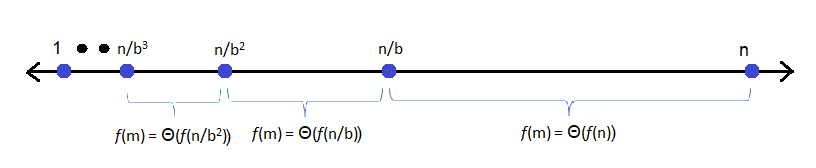
\includegraphics[width=\linewidth]{mastersTheorem.png}
  \caption{Shows $f{(m)}$ is in constant factor of $f{(n)}$}
\end{figure}
With Master theorem, we can represent recurrences within polylog factor for n as shown in figure 10.1.1, Other points are not covered. Hence, we need general form for covering all the points.

\begin{equation*}
T(n) = {a_1T({n \over b_1})} + {a_2T({n \over b_2})} + {a_3T({n \over b_3})}
\end{equation*}
Assume that $T(n) = n^p$, then
\begin{equation*}
\begin{split}
T(n) & = {a_1T({n \over b_1})^p} + {a_2T({n \over b_2})^p} + {a_3T({n \over b_3})^p} \\
& = [{a_1 \over {b_1}^p} + {a_2 \over {b_2}^p}  + {a_3 \over {b_3}^p}] . n^p
\end{split}
\end{equation*}

As per our initial assumption($T(n) = n^p$) the value of $[{a_1 \over {b_1}^p} + {a_2 \over {b_2}^p}  + {a_3 \over {b_3}^p}]$ should be 1.
We can find value of p by solving $[{a_1 \over {b_1}^p} + {a_2 \over {b_2}^p}  + {a_3 \over {b_3}^p}]$ = 1.\\

\section{General form: Akra-bazzi recurrence}

\begin{equation*}
T(x) = \begin{cases}
  \Theta(1)  &\text{$if 1 \leq x \leq x_0$}\\
    \sum_{i = {i}}^{k} a_iT({b_ix}) + g(x), &\text {$if x > x_0$ }
\end{cases}
\end{equation*}

where, 
\begin{enumerate}
    \item {$k \geq 1$} is an integer constant 
    \item {$a_i > 0$} is a constant for {$ 1 \leq i \leq k$}
    \item {$b_i \in $} (0,1) is a constant for {$1 \leq i \leq k$}
    \item {$x \geq 1$} is a real number
    \item {$x_0 \geq$} {$max \{{1 \over b_i} , {1 \over 1-b_i}$}\}
    \item g(x) is a non-negative function that satisfies a polynomial-growth condition.
\end{enumerate}

If can expand above recurrence as follows, \\  
    {$T(x) = a_1T(b_1x) + a_2T(b_2x) + a_3T(b_3x) + ... + a_kT(b_kx) + g(x)$}

\subsection{Polynomial-Growth condition}

We say that {$g(x)$} satisfies the polynomial-growth condition if there exist positive constants {$c_1$} and {$c_2$} such that for all {$x \geq 1$}, for all {$1 \leq i \leq k $}, and for all {$ u \in [b_ix,x]$}

\begin{center}
    {$c_1g(x) \leq g(u) \leq c_2g(x)$}
\end{center}

\begin{center}
    {$ i.e.\ \ \  g(u) = \Theta (g(x))$}
\end{center}

\subsection{The Akra-Bazzi Solution}

Consider the recurrence given in 10.2

\begin{equation*}
T(x) = \begin{cases}
  \Theta(1)  &\text{$if 1 \leq x \leq x_0$}\\
    \sum_{i = {i}}^{k} a_iT({b_ix}) + g(x), &\text {$if x > x_0$ }
\end{cases}
\end{equation*}

Let p be the unique real number for which {$ \sum_{i=1}^{k} a_i b_i^p = 1$} Then,

\begin{equation*}
T(x) = \Theta(x^p (1 + \int_1^x {g(u)\over u^p+1} du))
\end{equation*}


\section{Akra-Bazzi Solution}
\subsection{Deterministic Select}

For following recurrence, \\
\begin{equation*}
T'(n) = \begin{cases} \Theta(1):  &\text{$if n <140$}\\
    T'({n \over 5}) + T'({4n \over 5}) + \Theta(n) & \text{$if n \geq 140$}$
$\end{cases}

\end{equation*}

\begin{center}
a_1 = 1, b_1 = {1\over5}, a_2 = 1, b_2 = {4\over5} \\

a_1b_1^p + a_2b_2^p = 1

\end{center}
Putting values of a_1, b_1, a_2, b_2

\begin{center}
$  1 * {({1 \over 5})}^p + 1 * {({3 \over 4})}^p = 1 $
\end{center}

\begin{center}
$  {({1 \over 5})}^p + {({4 \over 5})}^p = 1 $
\end{center}
\begin{center}
p = 1  
\end{center}

putting value of p in Akra-Bazzi Solution,

\begin{center}
$T(n) = \Theta(n^1 (1 + \int_1^n {u\over u^2} du))$
\end{center}

\begin{center}
$T(n) = \Theta(n (1 + \int_1^n {1\over u} du))$
\end{center}

\begin{center}
$T(n) = \Theta(n (1 + [\ln u]_1^n)) $
\end{center}
\begin{center}
$T(n) = \Theta(n (1 + (\ln n - \ln 1))$
\end{center}
\begin{center}
$T(n) = \Theta(n\ln n)$
\end{center}

\subsection{Deterministic Select - 2}

For following recurrence, \\
\begin{equation*}
T'(n) = \begin{cases} \Theta(1)  &\text{$if n <140$}\\
    T'({n \over 5}) + T'({3n \over 4}) + \Theta(n) & \text{$if n \geq 140$}$
$\end{cases}

\end{equation*}

\begin{center}
a_1 = 1, b_1 = {1\over5}, a_2 = 1, b_2 = {3\over4} \\
\end{center}

Putting values of a_1, b_1, a_2, b_2 \\ 

\begin{center}
$  1 * {({1 \over 5})}^p + 1 * {({3 \over 4})}^p = 1 $
\end{center}

\begin{center}
{$ p < 1 $} 
\end{center}

putting value of p in Akra-Bazzi Solution,

\begin{center}
$T''(n) = \Theta(n^p (1 + \int_1^n {u\over u^p+1} du))$
\end{center}

\begin{center}
$T(n) = \Theta(n (1 + \int_1^n {1\over u^p+1} du))$
\end{center}

\begin{center}
$T(n) = \Theta(n (1 + [{u^{-p+1) \over -p1+1}]_1^n)) $
\end{center}
\begin{center}
$T(n) = \Theta({({1 \over 1-p})}^n - {({p \over 1-p})}^n n^p)$
\end{center}
\begin{center}
$T(n) = \Theta(n)$
\end{center}


\subsection{Examples of Akra-Bazzi recurrence}
\begin{enumerate}
    \item \textbf{{$T(x) = 2T{({x \over 4})} + 3T({3x \over 6}) + \Theta(x\log x)$}} \\

\begin{center}
a_1 = 2, b_1 = {1\over4}, a_2 = 3, b_2 = {1\over6} \\
\end{center}

Putting values of a_1, b_1, a_2, b_2 \\ 

\begin{center}
$  2 * {({1 \over 2})}^p + 3 * {({1 \over 6})}^p = 1 $
\end{center}

\begin{center}
{$ p = 1 $} 
\end{center}

putting value of p in Akra-Bazzi Solution,

\begin{center}
$T(x) = \Theta(x^1(1 + \int_1^x {u\ln u \over u^2} du))$
\end{center}

\begin{center}
$T(x) = \Theta(x(1 + \int_1^x {\ln u \over u} du))$
\end{center}

\begin{center}
$\int_1^u {\ln u \over u} du = \ln u \int_1^u {1 \over u} du - {\int_1^u {(\frac{d}{du} \ln u) \int_1^u {1 \over u} du}
$
\end{center}
\begin{center}
$2\int_1^u {\ln u \over u} du = (\ln u)^2$
\end{center}


\begin{center}
$\int_1^u {\ln u \over u} du = {(\ln u)^2 \over 2}$
\end{center}

\begin{center}
$T(x) = \Theta(x(1 + [(\ln u)^2]_1^x)) $
\end{center}

\begin{center}
$T(x) = \Theta(x(1 + [(\ln x)^2 - (\ln 1)^2])) $
\end{center}

\begin{center}
$T(x) = \Theta(x\log^2 x) $
\end{center}

Similarly, we can solve following recurrences,

\item \textbf{$T(x) = 2T{({x \over 4})} + 3T({3x \over 6}) + \Theta(x\log x)$} \\

\begin{center}
    p = 2 
\end{center}

\begin{center}
$T(x) = \Theta(x^2(1 + \int_1^x { {u^2\over \log u} \over u^3} du))$
\end{center}

\begin{center}
$T(x) = \Theta(x^2 \log\log x) $
\end{center}

\item \textbf{$T(x) = T{({x \over 2})} + \Theta(\log x)$} \\
\begin{center}
    p = 0 
\end{center}

\begin{center}
$T(x) = \Theta(x^0(1 + \int_1^x {\log u\over u} du))$
\end{center}

\begin{center}
$T(x) = \Theta(log^2 x) $
\end{center}

\item \textbf{$T(x) = {1 \over 2} T{({x \over 2})} + \Theta({1 \over x})$} \\
\begin{center}
    p = -1 
\end{center}

\begin{center}
$T(x) = \Theta({1 \over x}(1 + \int_1^x {1 \over u} du))$
\end{center}

\begin{center}
$T(x) = \Theta({log x \over x}) $
\end{center}

\end{enumerate}
\section{Summary}
\begin{enumerate}
    \item Revisited Deterministic Select.
    \item Revisited Master theorem.
    \item Akra-Bazzi theorem is generalization of masters theorem.
    \item We can map relation of p in Akra-Bazzi theorem and three cases in Master theorem as follows:
\begin{itemize}
    \item {$p > 1$} : Master theorem case 1 (might) 
    \item {$p = 1$} : Master theorem case 2
    \item {$p < 1$} : Master theorem case 3
\end{itemize}

\end{enumerate}
\end{document}